\documentclass{ximera}

\graphicspath{{./}{thePythagoreanTheorem/}{deMoivreSavesTheDay/}{complexNumbersFromDifferentAngles/}}

\usepackage{tikz}
\usepackage{tkz-euclide}
\usetkzobj{all}
\tikzstyle geometryDiagrams=[ultra thick,color=blue!50!black]
\newcommand{\tri}{\triangle}
\renewcommand{\l}{\ell}
\renewcommand{\P}{\mathcal{P}}
\newcommand{\R}{\mathbb{R}}
\newcommand{\Q}{\mathbb{Q}}

\newcommand{\Z}{\mathbb Z}

\renewcommand{\vec}{\mathbf}
\renewcommand{\d}{\,d}



%% Egyptian symbols

\usepackage{multido}
\newcommand{\egmil}[1]{\multido{\i=1+1}{#1}{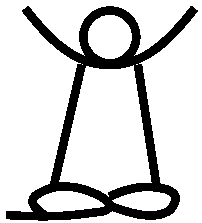
\includegraphics[scale=.1]{egyptian/egypt_person.pdf}\hspace{0.5mm}}}
\newcommand{\eghuntho}[1]{\multido{\i=1+1}{#1}{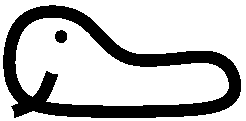
\includegraphics[scale=.1]{egyptian/egypt_fish.pdf}\hspace{0.5mm}}}
\newcommand{\egtentho}[1]{\multido{\i=1+1}{#1}{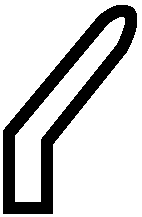
\includegraphics[scale=.1]{egyptian/egypt_finger.pdf}\hspace{0.5mm}}}
\newcommand{\egtho}[1]{\multido{\i=1+1}{#1}{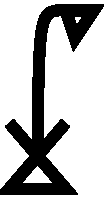
\includegraphics[scale=.1]{egyptian/egypt_lotus.pdf}\hspace{0.5mm}}}
\newcommand{\eghun}[1]{\multido{\i=1+1}{#1}{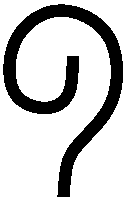
\includegraphics[scale=.1]{egyptian/egypt_scroll.pdf}\hspace{0.5mm}}}
\newcommand{\egten}[1]{\multido{\i=1+1}{#1}{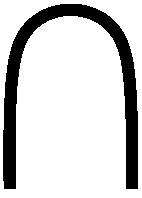
\includegraphics[scale=.1]{egyptian/egypt_heel.pdf}\hspace{0.5mm}}}
\newcommand{\egone}[1]{\multido{\i=1+1}{#1}{
\includegraphics[scale=.1]{egyptian/egypt_stroke.pdf}\hspace{0.5mm}}}
\newcommand{\egyptify}[7]{
 \multido{\i=1+1}{#1}{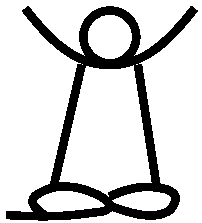
\includegraphics[scale=.1]{egyptian/egypt_person.pdf}\hspace{0.5mm}}
 \multido{\i=1+1}{#2}{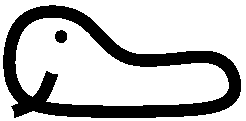
\includegraphics[scale=.1]{egyptian/egypt_fish.pdf}\hspace{0.5mm}}
 \multido{\i=1+1}{#3}{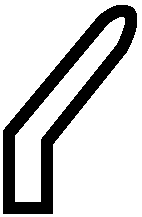
\includegraphics[scale=.1]{egyptian/egypt_finger.pdf}\hspace{0.5mm}}
 \multido{\i=1+1}{#4}{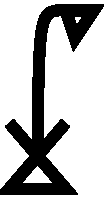
\includegraphics[scale=.1]{egyptian/egypt_lotus.pdf}\hspace{0.5mm}}
 \multido{\i=1+1}{#5}{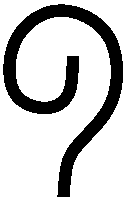
\includegraphics[scale=.1]{egyptian/egypt_scroll.pdf}\hspace{0.5mm}}
 \multido{\i=1+1}{#6}{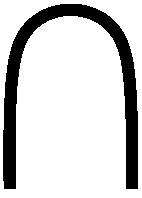
\includegraphics[scale=.1]{egyptian/egypt_heel.pdf}\hspace{0.5mm}}
 \multido{\i=1+1}{#7}{
\includegraphics[scale=.1]{egyptian/egypt_stroke.pdf}\hspace{0.5mm}}
 \hspace{.5mm}
}





\title{City geometry}
\begin{document}
\begin{abstract}
In this activity, we explore a geometry that is in some sense, nearly
euclidean.
\end{abstract}
\maketitle


One day I was walking through the city---that's right, New York City. I
had the most terrible feeling that I was lost. I had just passed a
\textit{Starbucks Coffee} on my left and a \textit{Sbarro Pizza} on my
right, when what did I see? Another \textit{Starbucks Coffee} and
\textit{Sbarro Pizza}! Three options occurred to me:
\begin{enumerate}
\item I was walking in circles.
\item I was at the nexus of the universe.\index{nexus of the universe}
\item New York City had way too many \textit{Starbucks} and \textit{Sbarro Pizzas}!
\end{enumerate}
Regardless, I was lost. My buddy Joe came to my rescue. He pointed out that the city is organized like a grid. 

``Ah! city geometry!'' I exclaimed.\index{city geometry}\index{geometry!City} At this point all Joe could say was
``Huh?''


\begin{question} What the heck was I talking about?
\end{question}

Let me tell you: \textit{euclidean geometry}\index{geometry!euclidean}
is regular old plane (not plain!) geometry. It is the geometry that
we've been exploring thus far in our journey.  In \textit{city
  geometry} we have points and lines, just like in Euclidean geometry.
However, most cities can be viewed as a grid of city blocks
\[
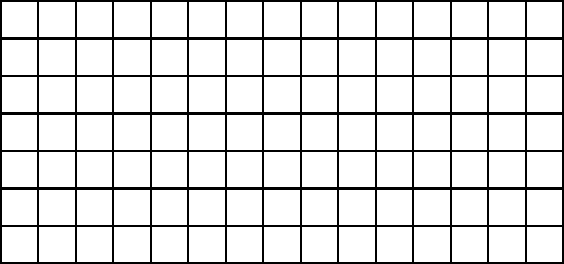
\includegraphics{citygrid.pdf}
\]
and when we travel in a city, we can only travel on the streets---we
can't cut through the blocks. This means that we don't measure
distance as the crow flies. Instead we use the \textit{taxicab
  distance}:

\begin{definition}\index{taxicab distance}\index{d@$d$!taxicab}\index{distance!taxicab}Given two points $A = (a_x,a_y)$ and $B = (b_x,b_y)$, we define the
\textbf{taxicab distance} as:
\[
d_T(A,B) = |a_x - b_x| + |a_y - b_y|
\]
\end{definition}


\begin{example} Consider the following points:
\[
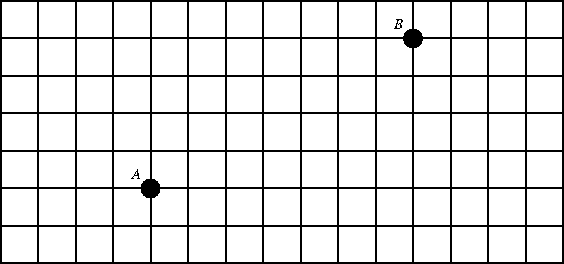
\includegraphics{citygrideg1.pdf}
\]
Let $A = (0,0)$. Now we see that $B = (7,4)$. Hence
\begin{align*}
d_T(A,B) &= |0 - 7| + |0-4|\\
&= 7 + 4 \\
&= 11.
\end{align*}
Of course in real life, you would want to add in the appropriate units
to your final answer.
\end{example}

\begin{question} How do you compute the distance between $A$ and $B$ as the crow flies?
\end{question}


\begin{definition}\index{city geometry}\index{geometry!city}
The geometry where points and lines are those from euclidean geometry
but distance is measured via taxicab distance is called \textbf{city
  geometry}.
\end{definition}

\begin{question} Compare and contrast the notion of a line in euclidean geometry and in city geometry. In either geometry is a line the unique shortest path between any two points?
\end{question}




\subsection{(Un)Common Structures}

How different is life in city geometry from life in euclidean
geometry? Let's find out!

\subsubsection{Triangles}

If we think back to euclidean geometry, we
may recall some lengthy discussions on triangles. Yet so far, we have
not really discussed triangles in city geometry.

\begin{question} What does a triangle look like in city geometry and how do you measure its angles? \index{city geometry!triangle}\index{triangle!city geometry}
\end{question}

I'll take this one. Triangles look the same in city geometry as they
do in euclidean geometry. Also, you measure angles in exactly the same
way. However, there is one minor hiccup. Consider these two triangles
in city geometry:
\[
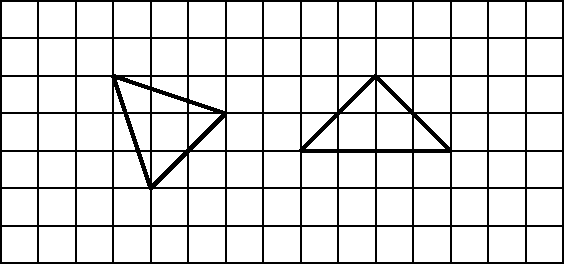
\includegraphics{citytri.pdf}
\]
\begin{question} 
What are the lengths of the sides of each of these triangles? Why is
this odd?
\end{question}
 

Hence we see that triangles are a bit funny in city geometry.

\subsubsection{Circles}

Circles are also discussed in many geometry courses and this course is
no different. However, in city geometry the circles are a little less
round. The first question we must answer is the following:

\begin{question} What is a circle?
\end{question}

Well, a circle is the collection of all points equidistant from a
given point. So in city geometry, we must conclude that a circle of
radius $2$ would look like:
\[
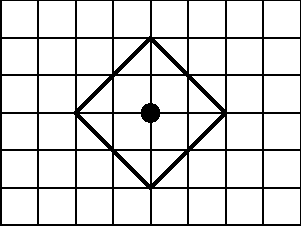
\includegraphics{citycircle.pdf}
\]
\index{circle!city geometry}\index{city geometry!circle}
\begin{question} What sort of shape should a city geometry compass draw?
\end{question}


\begin{question} 
How many points are there at the intersection of two circles in
euclidean geometry? How many points are there at the intersection of
two circles in city geometry?
\end{question}



\end{document}
